\documentclass{beamer}
\usepackage[utf8]{inputenc}
\usepackage[T1]{fontenc}

% blue theme
\usetheme{Madrid}

\title[	Interfejsy Komputer-Mózg]
{Interfejsy Komputer-Mózg}
\subtitle{Zastosowania w medycynie }
 
\author[Łukasz Klasiński] 
{ Łukasz Klasiński}
 
\institute[UWr]
{
  Wydział informatyki\\
  Uniwersytet Wrocławski
}

\date[18-12-2018]
{ Komunikacja człowiek-komputer }
 

\begin{document}
 
\frame{\titlepage}

\begin{frame}
\frametitle{Czym jest BCI?}

    \begin{block}{Definicja}<1->
        BCI (Brain-computer interface) jest komputerowym systemem, który pobiera, analizuje i tłumaczy sygnały mózgowe na polecenia, następnie polegając
        na urządzeniach zewnętrznych przeprowadza wybraną akcję. Jednak nie używa on zwykłych sygnałów wyjściowych mózgu, które
        wykorzystywane są podczas poruszania mięśniami. BCI działa mierząc sygnały pochodzące tylko z centralnego układu
        nerwowego. 
    \end{block}    
    \begin{exampleblock}{}<2->
        Często pomyłką jest mówienie, że BCI czyta w myślach - systemy te nie robią tego wyciągając informacje
        z użytkownika, ale umożliwiają mu interakcje z otoczeniem za pomocą sygnałów mózgowych, zamiast mięśni. Użytkownik 
        i BCI muszą razem współpracować i dopiero po odpowiednim treningu, użytkownik jest w stanie wygenerować zakodowane sygnały, 
        które BCI uczy się odszyfrowywać i tłumaczyć na odpowiednie polecenia do urządzenia wyjściowego.        
    \end{exampleblock}
\end{frame}

\begin{frame}
    \frametitle{Historia}

    \begin{itemize}
        \item <1->Pod koniec lat 60 praca z małpami pokazała, że sygnały z  neuronów kory mózgowej mogą być użyte do sterowania miernikiem igłowym.  
        \item <2-> pomysł zastosowania BCI w kontroli urządzeń takich jak protezy zostało przedstawione przez Jacques J. Vidal'a, który w 1973 roku przedstawił publikację o możliwości użycia takiego interfejsu przez ludzi.   
        \item <3-> W 1980 Elbert T. zademonstrował jak osoba za pomocą odczytów EEG kontrolowała pionowe ruchy zdjęcia na ekranie.
    \end{itemize}
\end{frame}

\begin{frame}
    \frametitle{Historia}
    \begin{itemize}
        \item <1-> 8 lat później Farwell LA. i Donchin E. pokazali jak używać sygnałów P300 aby wolontariusze, bez wcześniejszego wyszkolenia mogli wypisywać słowa na ekranie.
        \item <2-> Pod koniec lat 90 Wolpaw J.R. wytrenował wolontariuszy do kontrolowania kursora na ekranie za pomocą sygnałów mu.
        \item <3-> W 2006 roku pierwsza osoba z całkowitym paraliżem została podłączona do systemu BCI, który umożliwił jej otwieranie e-maili, sterowanie telewizorem oraz podstawowe akcje dłonią protezy.         
    \end{itemize}
\end{frame}
\begin{frame}
\frametitle{Historia}
\begin{center}
    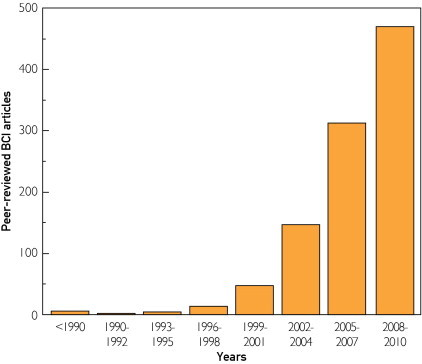
\includegraphics[scale=0.8]{chart.jpg}
\end{center}    
\end{frame}

\begin{frame}
    \frametitle{Pobieranie sygnałów}
        \begin{block}{}<1->
            Pierwsze BCI do pobierania sygnałów z mózgu użytkownika zwykle używały elektrod przyczepionych do skalpu.
            Niestety taka metoda pomimo bycia bezpieczną oraz tanią, odbiera zniekształcone sygnały, przez co tracona jest część informacji.
        \end{block}
        \begin{block}{}<2->
                Nowocześniejsze, bardziej precyzyjne systemy BCI do poprawnego działania wymagają inwazyjnej operacji w celu
                wszczepienia odpowiedniego implanta wprost do mózgu. Problemem jest jednak duże ryzyko powikłań, ograniczone
                pole odczytywania sygnałów oraz nieznane skutki długiego posiadania takich implantów.
        \end{block}
\end{frame}

\begin{frame}
    \frametitle{Komponenty BCI}
    \begin{center}
        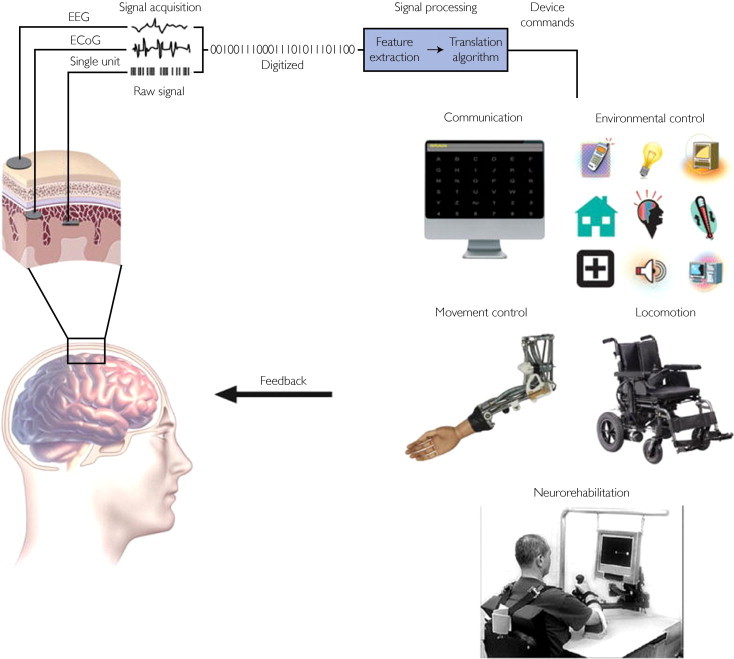
\includegraphics[scale=0.5]{comp.jpg}
    \end{center}    
\end{frame}

\begin{frame}
    \frametitle{Komponenty BCI}
    \begin{block}{1.Pobieranie sygnału}
        Sygnał jest pobierany za pomocą odpowiedniego sensora. Są one następnie odpowiednio wzmacniane do poziomów
        odpowiednich do przetwarzania przez elektronikę. Dodatkowo może on być odfiltrowany od szumów albo innych 
        sygnałów takich jak szum lini energetycznej. Następnie sygnał jest przetwarzany do postaci cyfrowej i wysyłany do komputera.   
    \end{block}
\end{frame}

\begin{frame}
    \frametitle{Komponenty BCI}
    \begin{block}{2.Wyodrębnianie cech}
        Wyodrębnianie cech jest procesem, który analizuje sygnał cyfrowy, aby odróżnić znany sygnał od obcego (czyli takie które sa rozpoznane jako polecenie
        dla BCI). Cechy te powinny mieć silną zależność od tego jakie są zamiary użytkownika. 
    \end{block}
\end{frame}

\begin{frame}
    \frametitle{Komponenty BCI}
    \begin{block}{3.Tłumaczenie cech}
        Wynikowe cechy sygnału są przekazywane do odpowiedniego algorytmu, który przekształca cechy na odpowiednie 
        polecenia dla urządzenia wyjściowego. Na przykład, zmniejszenie napięcia w konkretnej częstotliwości może być
        przetłumaczone jako ruch w górę kursora komputerowego. Algorytm ten powinien być się samodzielnie uczyć zmian w sygnale,
        aby zapewnić użytkownikowi jak największy, możliwy zasięg kontroli.  
    \end{block}
\end{frame}

\begin{frame}
    \frametitle{Komponenty BCI}
    \begin{block}{4.Urządzenie wyjściowe}
        Ostateczne komendy z algorytmu trafiają do urządzenia zewnętrznego umożliwiając kontrolę nad nimi. Następnie 
        urządzenie na którym operujemy przekazuje rezultat operacji do użytkownika, zamykając pętlę.
    \end{block}
\end{frame}

\begin{frame}
    \frametitle{BCI używające skalpu}
    Tego typu BCI umożliwiają kontrolę takich czynności jak:
    \begin{itemize}
        \item kontrola kursorów do 3 wymiarów
        \item urządzenia piszące
        \item protezy
        \item zdalną kontrolę nad wózkiem inwalidzkim
        \item przeglądanie internetu
        \item elektroniczne przewodniki dla osób ślepych
    \end{itemize}
\end{frame}

\begin{frame}
    \frametitle{BCI używające implantów}
    Tego typu BCI umożliwiają kontrolę takich czynności jak:
    \begin{itemize}
        \item kontrola poszczególnych palców, ręki oraz ramienia
        \item kontrola kursorów do 2 wymiarów
        \item bezpośredni tłumacz głosowy
        \item umożliwia stabilne odczytywanie sygnałów nawet po kilkunastu miesiącach
    \end{itemize}
\end{frame}

\begin{frame}
    \frametitle{Dostępne urządzenia komercyjne}
    Większość urządzeń BCI jest używana głównie w laboratoriach oraz do przeprowadzania różnych rehabilitacji.
    Z takich, które są dostępne do użytku domowego, możemy wymienić:
    \begin{itemize}
        \item Brainfingers, Emotiv, NeuroSky, są zestawami słuchawkowymi z wbudowanymi czujnikami, które umożliwiają
        kontrolowanie aplikacji, kilkunastu gier
        \item BrainMaster, Mindballm, EGGInfo, mają mają poprawiać skupienie i koncentrację. 
        \item IntendiX - EGG BCI system, który pozwala na zdalne pisanie wiadomości oraz posiada syntezator głosowy.
    \end{itemize}
\end{frame}


\begin{frame}
    \frametitle{Przykładowe urządzenia}
    \begin{center}
        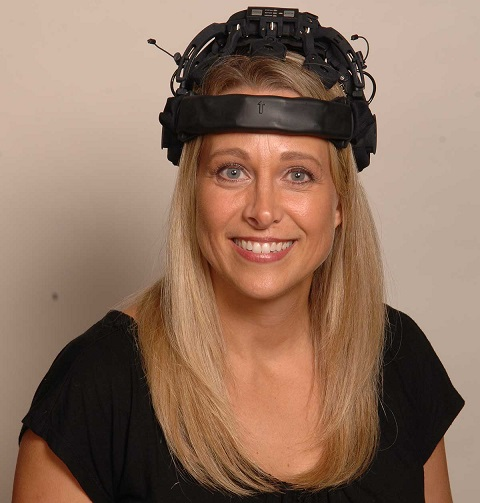
\includegraphics[scale=0.5]{freedom.jpg}
        \\

        {\tiny freedom headset }
    \end{center}    
\end{frame}

\begin{frame}
    \frametitle{Przykładowe urządzenia}
    \begin{center}
        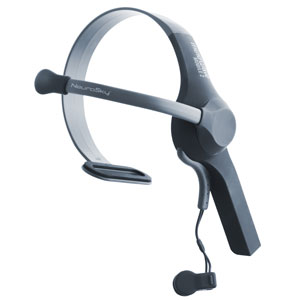
\includegraphics[scale=0.5]{mindwave.jpg}
        \\

        {\tiny mindwave headset }
    \end{center}    
\end{frame}

\begin{frame}
    \frametitle{Przykładowe urządzenia}
    \begin{center}
        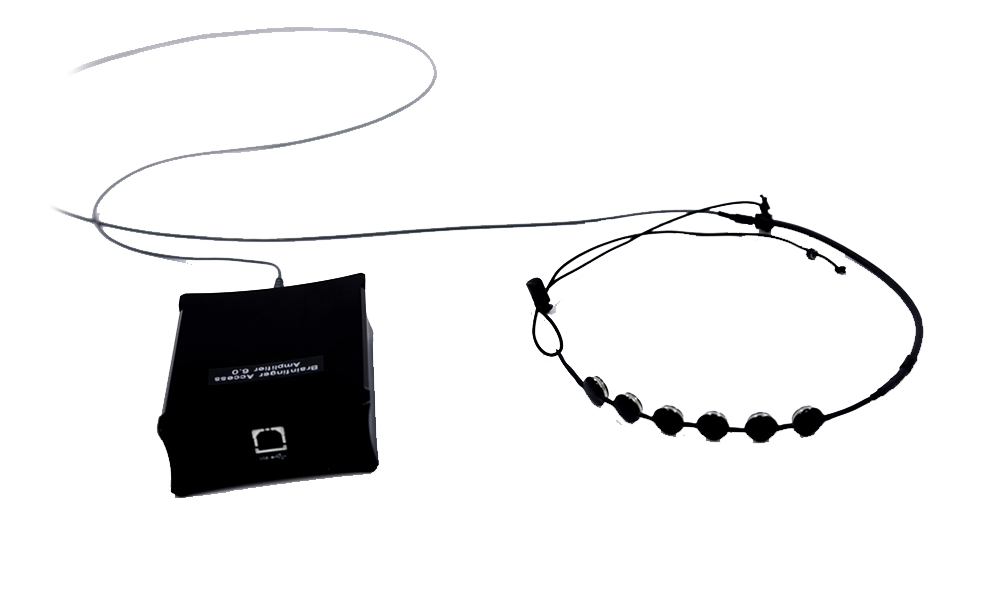
\includegraphics[scale=0.3]{fingers.png}
        \\

        {\tiny brainfingers headset }
    \end{center}    
\end{frame}


\begin{frame}
    \frametitle{Przykładowe urządzenia}
    \begin{center}
        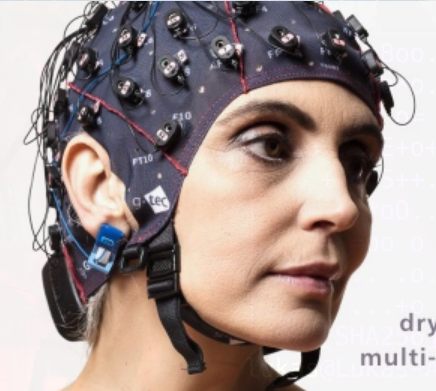
\includegraphics[scale=0.5]{nautillus.png}
        \\

        {\tiny nautilus headset }
    \end{center}    
\end{frame}

\begin{frame}
    \frametitle{Przyszłość BCI}
    \begin{itemize}
        \item polepszone urządzenia EEG
        \item wszczepialne elektrody, które są bezpieczne i mogą działać przez lata
        \item zmniejszenie kosztów wszczepienia implantów
        \item zapewnienie niezawodności oraz prostoty obsługi na poziomie naturalnej kontroli mięśni
        \item przystosowanie się BCI do użytkownika bez specjalnego trenowania 
    \end{itemize}
\end{frame}

\begin{frame}
    \frametitle{Fin}
    \begin{center}
    Dziękuję za uwagę!
    \end{center}
    \mbox{}
    \vfill
    \begin{center}
        {\tiny Opracowano na podstawie artykułu Jerry J. Shih, Dean J. Krusienski oraz Jonathana R. Wolpaw 'Brain-Computer Interfaces in Medicine'}
    \end{center}
\end{frame}


\end{document}